\documentclass[]{article}
\usepackage[utf8]{inputenc}
\usepackage[russian]{babel}
\usepackage{amsmath}
\usepackage{graphicx}
\hoffset=-100pt
\voffset=-100pt
\textwidth=520pt
\textheight=700pt
%а тут уже можно что-нибудь менять.
\title{The bus-driver-planning challenge}
\author{Ошканов В.С. гр. 13122}
\begin{document}
\maketitle
\section{Математическая модель}

Я решаю задачу о составлении расписания водителей автобусов с
сайта https://careers.quintiq.com/puzzle.html
Целью задачи является составление расписания с максимальной
суммой бонусов и штрафов, обозначенных в задании.

Для записи математической модели нам потребуются следующие обозначения:
\par
\textit{Множества}:
\par\noindent
$I = \{1,...,11\}$ --- множество водителей.
\par\noindent
$J = \{1,...,14\}$ --- множество дней.
\par\noindent
$K = \{1,2,3\}$ --- множество маршрутов.
\par
\textit{Параметры}:
\par\noindent
$d_{ij}$ --- (d - day off) равeн 1, если у водителя $i$ выходной в день $j$, и 0
в противном случае, $i\in I$, $j\in J$.
\par\noindent
$pd_{ij}$ --- (pd - prefer day off) равен 1, если водитель $i$ хочет отдыхать в
день $j$, $i\in I$, $j\in J$.
\par\noindent
$pe_{ij}$ --- (pe - prefer early) водитель $i$ хочет работать в утреннюю
смену в день $j$, $i\in I$, $j\in J$.
\par\noindent
$pl_{ij}$ --- (pl - prefer late) водитель $i$ хочет работать в вечернюю
смену в день $j$, $i\in I$, $j\in J$.
\par\noindent
$can_{ik}$ --- квалификация водителя $i$ позволяет ему работать на маршруте $k$,
 $i\in I$, $k\in K$.
\par
\textit{Переменные}:
\par\noindent
$e_{ijk}$ --- равна 1, если водитель $i$ работает в день $j$ на маршруте $k$
в утреннюю смену.
\par\noindent
$l_{ijk}$ --- равна 1, если водитель $i$ работает в день $j$ на маршруте $k$
в вечернюю смену.

Далее следует набор бинарных переменных, необходимых для составления модели:
\par\noindent
$earlyafterlate_{ij}$ - равна 1, если у водителя утренняя смена следует за вечерней,
$i \in I, j \in J\backslash\{14\}$.
\par\noindent
$earlyshiftspare_{jk}$ - равна 1, если в день $j$ на маршруте $k$ нет водителя в утреннюю смену.
\par\noindent
$lateshiftspare_{jk}$ - равна 1, если в день $j$ на маршруте $k$ нет водителя в вечернюю смену.
\par\noindent
$morethanfourdays_{i}$ - равна тому, насколько больше, чем 4,  вечерних смен водитель $i$ выполняет за все дни.
\par\noindent
$lessthanfourdays_{i}$ - равна тому, насколько меньше, чем 4,  вечерних смен водитель $i$ выполняет за все дни.
\par\noindent
$threedaysoff_{i \in I, j \in J}$ - водитель $i$ имеет 3 выходных подряд, начиная с дня $j$.
\par\noindent

С использованием введенных обозначений, математическая модель задачи о рационе
запишется следующим образом:
\begin{eqnarray}
-4 * \sum_{i\in I}\sum_{j\in J}(pd_{ij}*\sum_{k \in K}(e_{ijk}+l_{ijk}))
-8 * \sum_{i\in I}(morethanfourdays_i+lessthanfourdays_i) \\ \nonumber
-30 * \sum_{i\in I}\sum_{j \in J\backslash\{14\}} earlyafterlate_ij
-20 * \sum_{j \in J}\sum_{k \in K} (earlyshiftspare_{ik} + lateshiftspare_{jk}) \\ \nonumber
+ 3 * \sum_{i \in I}\sum_{j \in J}\sum_{k \in K} (pe_{ij}*e_{ijk} + pl_{ij}*l_{ijk})
+ 5 * \sum_{i \in I}\sum_{j \in J\backslash{13,14}} threedaysoff_{ij}\rightarrow\max;
\end{eqnarray}
\begin{equation}\label{spare1}
  \sum_{i \in I} e_{ijk} + earlyshiftspare_{jk} = 1, j \in J, k \in K.
\end{equation}
\begin{equation}\label{spare2}
  \sum_{i \in I} l_{ijk} + lateshiftspare_{jk} = 1, j \in J, k \in K.
\end{equation}
\begin{equation}\label{one1}
  \sum_{k \in K} e_{ijk} \leq 1, i \in I, j \in J.
\end{equation}
\begin{equation}\label{one2}
  \sum_{k \in K} l_{ijk} \leq 1, i \in I, j \in J.
\end{equation}
\begin{equation}\label{do1}
  \sum_{k \in K} e_{ijk}*d_{ij} = 0, i \in I, j \in J.
\end{equation}
\begin{equation}\label{do2}
  \sum_{k \in K} l_{ijk}*d_{ij} = 0, i \in I, j \in J.
\end{equation}
\begin{equation}\label{3days}
  \sum_{n = j}^{j+2}\sum_{k \in K} l_{ink} \leq 3, i \in I, j \in J\backslash\{13,14\}.
\end{equation}
\begin{equation}\label{earlyafterlate}
  \sum_{k \in K} (e_{i j+1 k} + l_{ijk})
              - earlyafterlate_{ij} \leq 1, i \in I, j \in J\backslash\{13\}.
\end{equation}
\begin{equation}\label{oneshift}
  \sum_{k \in K} (e_{ijk}+l_{ijk}) \leq 1, i \in I, j \in J.
\end{equation}
\begin{equation}\label{mtf}
  \sum_{j \in J}\sum_{k \in K} l_{ijk} - morethanfourdays_{i} - 4 \leq 0, i \in I.
\end{equation}
\begin{equation}\label{ltf}
  \sum_{j \in J}\sum_{k \in K} l_{ijk} - lessthanfourdays_{i} - 4 \geq 0, i \in I.
\end{equation}
\begin{equation}\label{can1}
  e_{ijk}*(1-can_{ik}) = 0, i \in I, j \in J, k \in K.
\end{equation}
\begin{equation}\label{can2}
  l_{ijk}*(1-can_{ik}) = 0, i \in I, j \in J, k \in K.
\end{equation}
\begin{equation}\label{tdo1}
  \sum_{k \in K} (e_{ijk}+l_{ijk}+e{ij+1k}+l_{ij+1k}+e_{ij+2k}+l_{ij+2k})
        + 3*threedaysoff_{ij} \leq 3, i \in I, j \in J\backslash\{13,14\}.
\end{equation}
\begin{equation}\label{tdo2}
  \sum {j \in  J\backslash\{13,14\}} threedaysoff_{ij} \leq 1.
\end{equation}

Ограничения \eqref{spare1} и \eqref{spare2} нужны для правильной
 инициализации переменных $earlyshiftspare$ и $lateshiftspare$.

Ограничения \eqref{one1} и \eqref{one2} нужны, чтобы водитель не
мог работать на двух линиях одновременно.

Ограничения \eqref{do1} и \eqref{do2} задают выходные.

Ограничения \eqref{3days} ограничивают количество подряд идущих вечерних
смен. Я решил сделать их обязательными, а не выносить в целевую функцию,
для обеспечения большей производительности, поскольку невыполнение этого
условия даёт большой штраф.

Ограничения \eqref{oneshift} необходимы для того, чтобы водитель работал только одну
смену в день.

Ограничения \eqref{mtf} и \eqref{ltf} задают переменные $morethanfourdays$ и
$lessthanfourdays$, а ограничения \eqref{can1} и \eqref{can2} нужны для соблюдения
квалификации.

И наконец, ограничение \eqref{tdo1} и \eqref{tdo2} задают переменные $threedaysoff$.
\section{Вычислительный эксперимент}
Я ввёл данные в GLPK, запустил, и начал ждать. Ждал, ждал, сходил погулять, ещё подождал,
после чего понял, что модель нужно что-то менять. Сначала я нашёл в опциях запуска
GLPK опцию --pcost (branch using hybrid pseudocost heuristic (may beseful for hard instances)).
С ней GLPK начал работать правда довольно быстрее, но всё же, со всеми ограничениями
модель считалась необозримое время.  Тогда я добавил новое ограничение:
\begin{equation}
  treedaysoff_{ij}*(1-d_{ij}-d_{ij-1}-d_{ij-2}) \leq 0, i \in I, j \in \{3..12\}.
\end{equation}

Это условие нужно для того, чтобы рассматривать в качестве дней "кандидатов" на
начало трёхдневного отдыха только те дни, которые являются выходными, или перед
ними, или после них есть выходной. Это сокращает множество допустимых решений,
и тем самым ускоряет работу GLPK.

В итоге, у меня получился результат 93.8\%, что, как я считаю, очень даже неплохо.

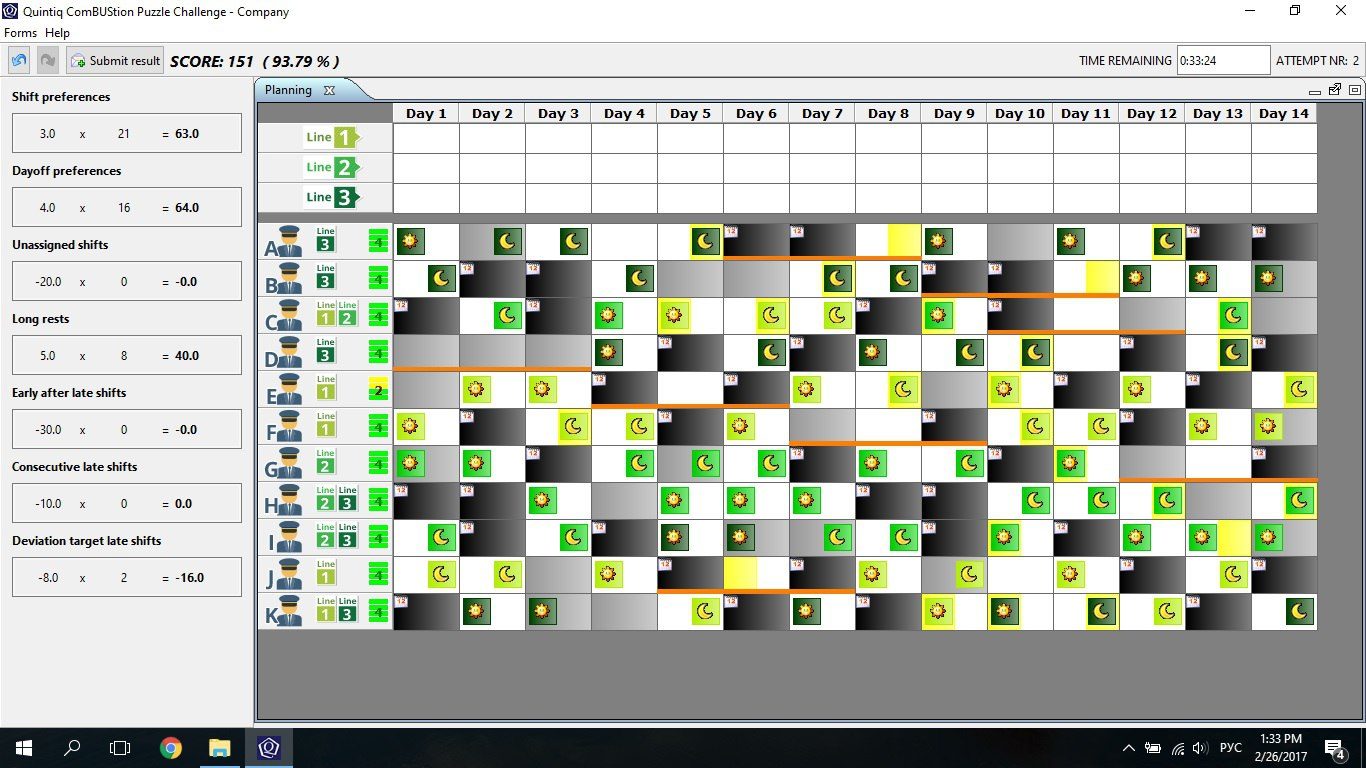
\includegraphics[scale=0.5]{bus_res.jpg}
\section{Вывод}
Линейное программирование очень облегчает составление расписаний, но мне так
и не удалось составить модель, дающая результат 100\% за разумное время.
\end{document}
